
\section{Related work}
The Master thesis written by Anders Vinther and Magnus Vinther from Aarhus university, describes the various methods used for path finding in 2D worlds. Reading the thesis gave a great overview of the different algorithms and methods related to doing path finding both for grid based worlds and polygonal worlds.
\cite{vinther2015pathfinding}
In the paper Wayfinding \cite{wayfinding} which is a DTU project in collaboration with Dalux, the goal was to do path finding for a person in a building. This is similar to what will be done in this thesis and therefore their report had some good thoughts on how to initially go about this problem. Even though this project ended up being implemented in a different way using a grid based world as opposed to their polygonal world system, their report still made a good catalyst for this project.
A good amount of time during this project was spent considering whether to go about this problem using a grid based world or a polygonal world structure. This was an important crossroad that came early in the project, and would lead to different implementations and methods used. The decision was changed a few times during this project as more insights came. Two papers gave some inspiration to these different ways to approach the problem. 
%In this paper \cite{xu2017bim} they use BIM data in the IFC format to do 2D indoor path-planning for humans. They do this using a grid based world system.
In this paper \cite{xu2017bim} they have the goal of solving quote “Accurate and efficient indoor path planning” in BIM models. The way they have implemented it is by using the grid system. 

%\begin{figure}[H]
%    \centering
%    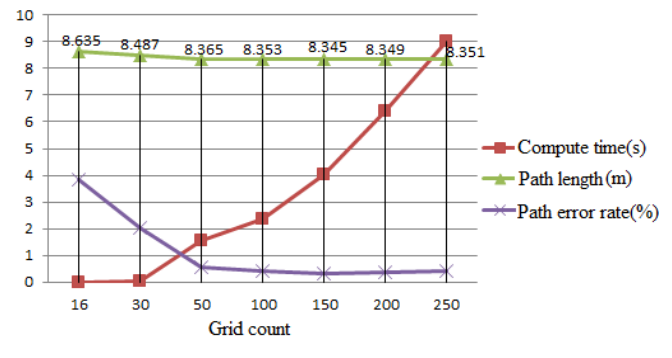
\includegraphics[width=1\textwidth]{fig/graph_grid_system.PNG}
%    \caption{Graph showing computation cost as a function of grid count~\cite{xu2017bim}}
%    \label{}
%\end{figure}

%They show what happens with the computation time when increasing the number of nodes. And also shows how minimal an effect it has on the path length.

%\begin{itemize}
%    \item Explain visibility graphs
%    \item Explain that different approaches had been used in the past, literature review, include articles.
%\end{itemize}

\begin{figure}[H]
    \centering
    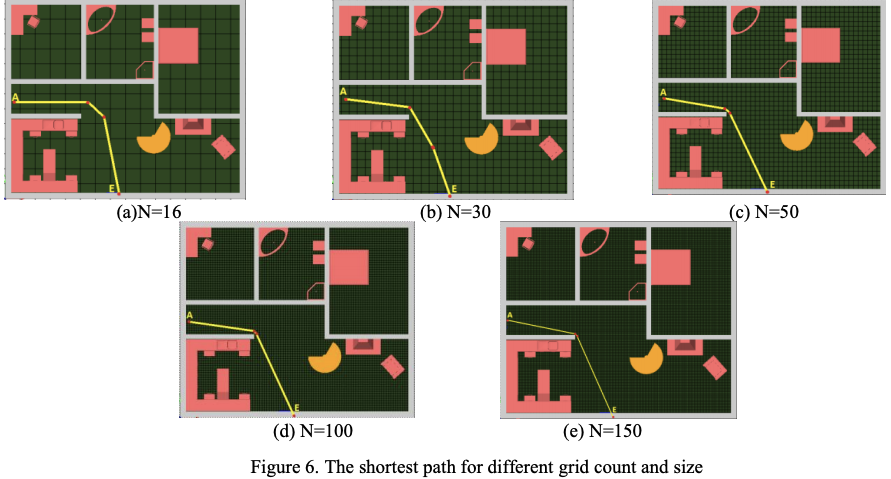
\includegraphics[width=1\textwidth]{fig/report/grid_fra_paper.png}
    \label{}
    \caption[]{Grid from paper}
\end{figure}
A paper that decided not to use the grid based system was this paper \cite{lee2010computing}. They chose a graph connectivity approach to indoor pathfinding.
\begin{figure}[H]
    \centering
    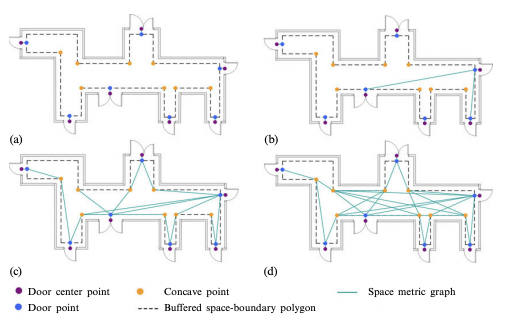
\includegraphics[width=1\textwidth]{fig/report/graph_connectivity_paper.png}
    \label{}
    \caption[]{Graph connectivity paper}
\end{figure}
The two papers illustrated that both the grid based world and the graph connectivity world were reliable approaches to take for doing path finding.

\section{Spot}
%Hvad er cad modeller og robotten.
%Giv en kontekst.
%Hvorfor er vi interesseret i at løse problemet.
The Spot robot is produced by Boston Dynamics and is their first commercially available robot currently being sold for a minimum of 74.500 dollars \cite{spot}. Spot is a quadruped that resembles a dog. It can be controlled with a tablet controller, but it can also be programmed to do autonomous tasks. This can be done using Spot's own Python SDK. The purpose of Spot is according to Boston Dynamics the following: "Spot Explorer is designed for developers eager to explore how flexible mobile robots can be adapted for tasks ranging from industrial inspection to entertainment."\cite{spot}

Industrial inspection is precisely what Spot will be used for in this project. Although this project does not work with Spot directly the project does take into consideration it's dimensions and capabilities when programming the path. The actual programming of Spot to walk the path programmed in this project, will be something for a future project. \ref{Future_work}

One of Spot's more useful properties is obstacle avoidance. Say we tell Spot to go from a point x to another point y - either by using it's controller or by a programmed path - if there is an object that blocks the straight path between point x and point y, Spot will be able to detect this object and move around it. 
This is a useful feature because it allows us to program a path for Spot without having to worry about it bumping into objects that would stand it its way such as furniture or construction tools.
Spot can also walk up and down stairs which will also be interesting for future development of this project, allowing it not only to walk around one floor but multiple floors.

\begin{itemize}
    \item Write about its length and width.
\end{itemize}

\begin{figure}[H]
    \centering
    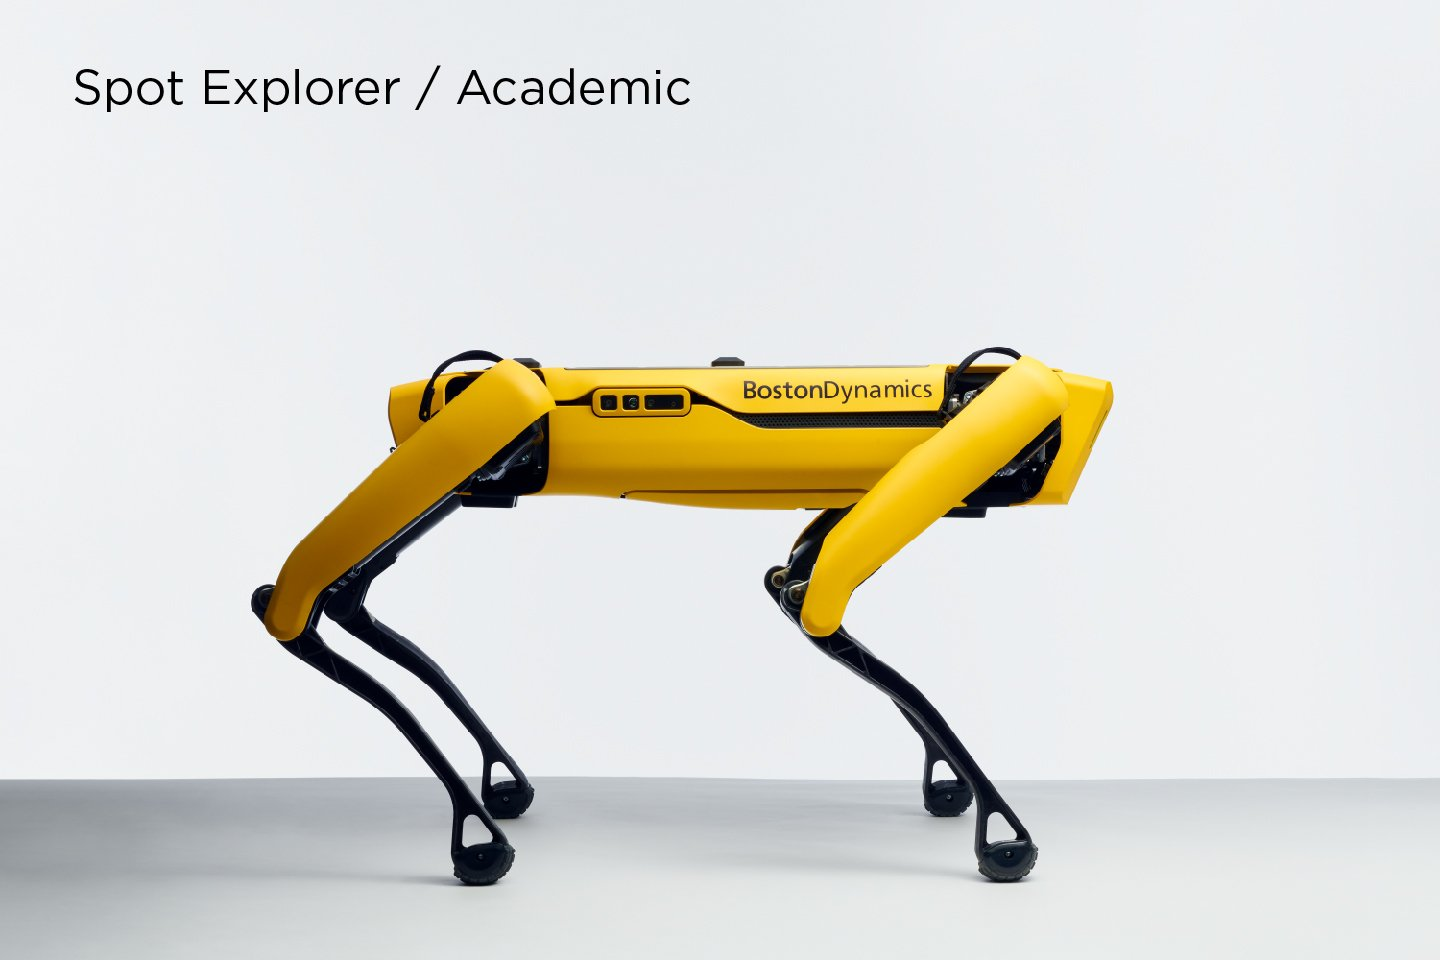
\includegraphics[width=1\textwidth]{fig/report/Spot Explorer-1.jpeg}
    \label{}
    \caption[The SPOT robot]{The Spot robot\textbf{}~\cite{spot}}
\end{figure}



\section{Data set}\label{dataset}
This project works with Building Information Modeling (BIM) data. 
The difference between Computer Aided Design (CAD) and BIM is that there is semantic information associated with each element in BIM data. In CAD a line is a line while in BIM a line can have the properties of being a wall. Not only that you can have all the parameters and properties of the wall associated with it.
\cite{bim_vs_cad}
BIM data goes beyond capturing just the geometric information, it also captures the semantic information associated with the building which allows it to better model reality. %This is why it was made mandatory in Denmark.
There are different formats for BIM data but the format of the data used in this thesis is the Industry Foundation Classes (IFC) format, which is the official international standard format for BIM models. 



\begin{comment}
In the data The coordinates are given in a polygonal triangle structure. This means that the floor plan is drawn from these coordinates by a mesh of triangle polygons. Each room from in the floor plan consists of its own tree branch, which makes it easy to include or exclude rooms in the floor plan.


The data set used in this project consists of html code of the room coordinates and the door coordinates in the format of the file is IFC (Industry Foundation Classes). [insert reference: https://fileinfo.com/extension/ifc]
[Insert picture of data]
Describing rooms and floor plans with triangle forming coordinates is a common way and makes sense for many reasons.
(Insert article reference that describes this way of plotting rooms)
(Insert picture of floor plan with triangles).
\\
The door coordinates also consists of the set of 3 coordinates with a x,y and z coordinate. Where the z coordinate says how tall the door is. 
\\
BIM models is also available for use, but will not necessarily be used since we start by modelling in 2D.
(Describe BIM models)
\begin{itemize}
    \item Write the format of the code
    \item Triangulation of the coordinates makes up the room
    \item Write about door information
\end{itemize}

Ifc is primary standard for BIM models
IFC is a schema not a format 
https://bimconnect.org/en/software/what-is-ifc/
Great interoperativebility
IFC format is compulsoary in Denmark for publicly aided building projects
IFC xml is less used for bigger buildings
object based inheritance hierachy

%In IFC open shell you it still wouldn't be a piece of cake
%probably have to take care of the triangulation on your own perhaps..
Since it is only simple version of IFC with simple objects I can use my own loader.
.
"The BIM approach is to use actual elements to represent real-world"
components.
Revit is designed for bim models.
CAD can be used for the design of everything from iphones to buildings.
BIM is a designing pattern focused for buildings only.

"Basically, when using CAD for building design, you focus on creating drawings. When using BIM, you focus on creating a building model and then the drawings can be generated from the model. "

https://knowledge.autodesk.com/support/revit-products/learn-explore/caas/video/youtube/lesson/143344-courseId-100332.html

This is the autodesk handbook on IFC format.
https://damassets.autodesk.net/content/dam/autodesk/draftr/2528/180213_IFC_Handbuch.pdf

\end{comment}






\section{Graph Theory}
As explained in the objective section \ref{Objective} of the introduction a big part of this project relies on the use of graphs, therefore graph theory plays a big role in this project. 
The program is essentially representing the building using two graphs.%, where one is a subgraph of the other. 
For the first graph the building is discretized and sampled in a grid. Each grid point is in this graph represented by a node. This will be called the "grid"-graph.
For the second graph each room of the building is represented as a node. This is called the "room"-graph.
In the following sections the relevant graph theory will be explained, which will form a basis for the Travelling salesman algorithm used to solve the path finding problem.


\subsection{What are graphs?}
Graphs are used in a wide variety of different fields to model networks and in general connections between different objects. This could for example be in electrical networks to model the relationship between resistors and capacitors or in social sciences to model connections between human beings.

A graph can be formulated as a function of nodes and edges.
$G(n,e)$
[insert picture]
A graph can be directed or undirected. With a directed graph the edge between two nodes represent a one way connection, the edge is thereby "directed" from one node to another. In an undirected graph there is no general direction meaning you can go from node a to node b and from node b to node a. In this project the program works with undirected graphs since if there is a connection between two rooms it is assumed that Spot can walk from room a to room b the same way it can walk from room b to room a, and the cost of the walk will also be identical [chapter 10 \cite{bondy1976graph}].

The edges of the graph can also be weighted or unweighted. In this project the program works with weighted edges where the weights of the edges are equal to the euclidean distance between the two nodes.



\subsection{Connectivity}
The approximate solution to the traveling salesman problem used in this program - explained further in \ref{TSP} - has a prerequisite that the graph used is fully connected - also defined as complete.  
Connectivity is a measure of how connected the nodes of the graph are. A minimal connected graph is a graph that if one of the edges is removed the graph will become disconnected. A fully connected or complete graph is a graph where every node has an edge to every other node in the graph. [insert picture of the two examples.] chapter 3 \cite{bondy1976graph}


\section{Minimum spanning tree}
Another concept needed to solve the Traveling salesman problem is the minimum spanning tree (MST). The idea behind minimum spanning tree is to find a minimal connected graph with the minimum summed edge weights. For a given graph there can be multiple minimum spanning trees since different trees can have the same minimum summed edge weights. chapter 23\cite{cormen2009introduction}

There exist different algorithms to find the minimum spanning tree of a graph. In this program the minimum spanning tree is found using the build in function in the networkx library. This function uses Kruskals algorithm to find the minimum spanning tree. chapter[23.2]\cite{cormen2009introduction}


\section{Shortest path problem} 
Before finding the minimum spanning tree another important thing to do is to find the minimum distance between two nodes in a graph. We want to find the minimum distance between all room nodes and use the distance as the weight of the edges between the nodes. This way we will have the complete "room" graph and can from there start solving for the traveling salesman problem.

There exist different shortest path algorithms. The one chosen in this project is the A star algorithm, which is an optimal algorithm, meaning it guarantees to find the shortest path. \cite{A_star} 

The A star algorithm works by using information about how far a node is from the start node and how far away it is from the end node to assess which direction to move in. When deciding on which direction to move it evaluates each neighbour cell their g(n)-cost, h(n)-cost and f(n)-cost. The g(n)-cost 
is the cost from the start node to node n, the h-cost is the cost from node n to the end node, measured with some measurement heuristic, like the euclidean distance for example. The f(n) cost is the sum of the g(n) cost and the h(n) cost. The algorithm moves to the node with the lowest f(n) cost.

[insert sketch]
%\begin{itemize}
%    \item Explain briefly how it works.
%\end{itemize}
%Again the Networkx framework has a built in function for the A star algorithm.





\section{Spatial Data structures}
Spatial data structures are data structures that store objects and the geometric information associated with the object. The objects are stored at the leaf nodes of a tree-structure where the branches of the tree indicate separation in space. chapter 1. \cite{laurini1992fundamentals}. [insert figure] %The searching algorithm used in this project is the nearest neighbour algorithm.
The main use of spatial data structures in this project is to quickly find the nearest objects to a given node. This could for example be to find the closest wall to a given node. Having a data structure that allows for fast access to nearby objects can drastically speed up the program, since the alternative method would be a brute force approach where each object would have to be checked to find the nearest object.


There exist different spatial data structures but most of these work only with point objects. This is for example the case with  KD-tree, which is a binary tree that for every branch splits space in two and has point objects at the leaf nodes. \cite{bentley1975binarysearch}. 

In this project we are interested in storing multidimensional objects - such as walls and rooms - as well as point objects and we are therefore interested in using a spatial data structure that allows for storage of such multidimensional objects.

One spatial data structure that meets these criteria is the R-tree.

%\begin{itemize}
    %\item Explain more about spatial data structures and their uses especially in graphics.
%\end{itemize}

\section{R-tree}
R-tree is an abbreviation for rectangle tree which is a suitable name since it works by making a bounding box - bounding volume in 3D - around the objects in a hierarchical structure. \cite{guttman1984r}. When a query is made the R-tree checks which of the bounding boxes at the top layer intersects with the bounding box of that query, and then goes a level deeper on the branch of the bounding box it intersected with. I keeps doing this until it hits the leaf nodes or until the bounding box of the query does not intersect with any of the rectangles in the given layer.
 
To illustrate how this hierarchical structure works take for example the  elements in a house. At the top level we have the house itself. Inside the house we have different rooms, each of which can be bounded by a box. Inside each of the rooms we have the furniture which can also be bounded by a box. When a query is made the R-tree first checks if the query intersects with the bounding box of the house. If this is the case it checks which of the rooms it intersects with and so on. In this way the R-tree returns the objects that are closest to the query. 




%\section{Grid data vs visibility graph}
%To make the robot walk from one room to another or one place in the building to another, it is important to understand  and decide on a way to implement the connectivity between the rooms. There are mainly two different kinds of implementations; a graph connectivity implementation and a grid implementation.

%The grid implementation works by discretizing the floor of the building into a grid with nodes of a specific size; the smaller the node size the higher the resolution of the grid.

%The graph connectivity approach works by representing each room/area by a node/dot which will be connected by a line to other rooms in the floor.

%The different implementations have different advantages and limitations. For example computationally the graph connectivity approach is much more scalable with bigger buildings or construction sites where as implementing a grid system in these situations will be more taxing computationally since a lot of nodes will have to be calculated. 

%On the other hand the advantage of the grid method is that its pathfinding algorithms will work on all building shapes. 
%Imagine the floor plan of the building below:


%\begin{figure}[H]
%    \centering
%    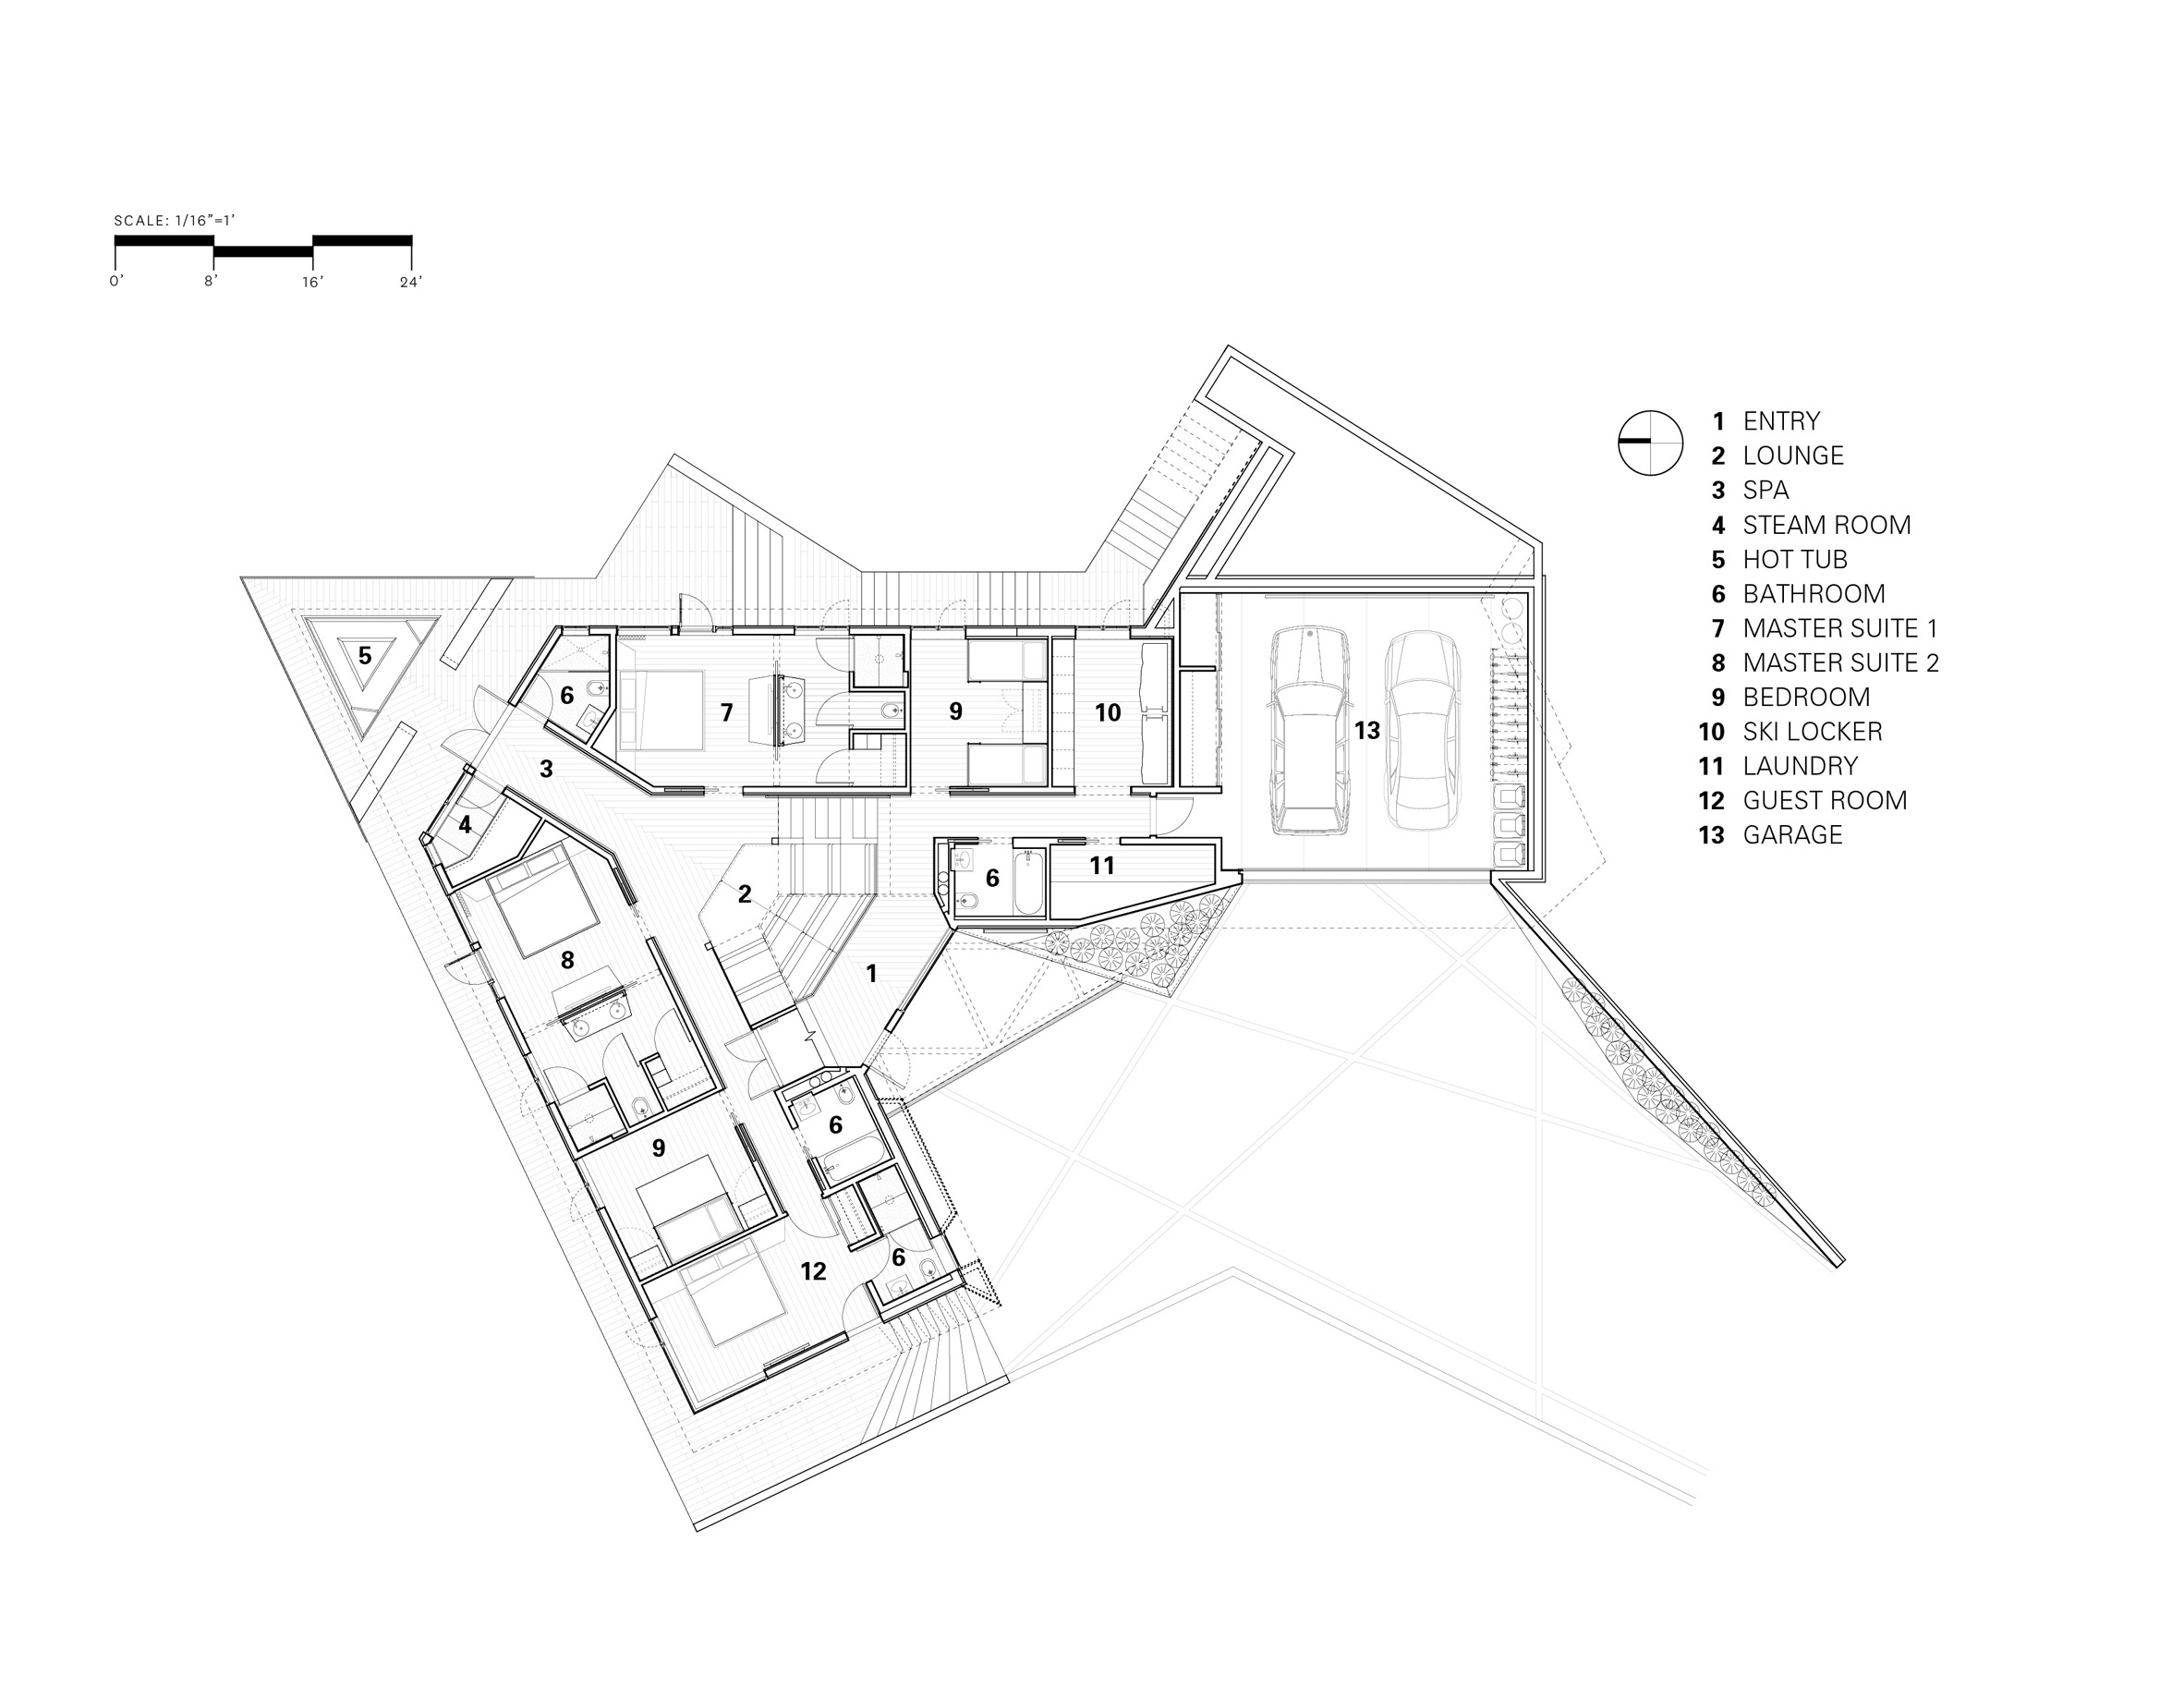
\includegraphics[width=1\textwidth]{fig/weird_floorplan.png}
%    \label{}
%    \caption[Weird floor plan]{Weird floor plan~\cite{weird_building}}
%\end{figure}

%When using a grid system apporach it will be possible to get an agent to walk from area 12 to 13 by specifically telling it which nodes are walkable and which nodes are not e.g walls. This will not be possible for the graph connectivity graph. The graph will here see only that area 12 and 13 are connected but not in which way. The method will draw a straight line between the two points and not see that the areas in reality are connected by the long pathway that goes through the entire floor plan.





\section{Distance field}
Which nodes in the building that Spot can traverse and which it can not traverse is determined with the use of distance fields. 
The distance field works with a grid based graph systems. There are different variations of the distance field \cite{distance_field} but the one used in this program is a distance field where each node in the grid is associated with an attribute that indicates the euclidean distance to the nearest wall. This attribute is then used to remove nodes that are too close to their nearest wall allowing for a realistic buffer space between Spot and the walls of the building. This is also known as a Boolean distance field.


%When humans walk around in a building we don't walk right next to the wall, scraping our shoulder to the wall (unless the path is very narrow) the same should be the case for the robot. If there was no buffer zone in front of the walls of the building, one could imagine that when Spot would have to turn a corner the program would tell it to walk right alongside the wall since this would allow for the shortest path to turn the corner.

%Making use of the distance field is the entire reason the grid structure of the graph was chosen over the visibility graph structure.

%The distance field allows for certain advantages that makes it a very robust solution. It is a robust solution because it for all nodes in the grid indicates whether Spot can traverse the node or not. This makes the approach useful for all kinds of obscure buildings.  


\section{Ray casting algorithm}
Figuring out which room each node in the grid belongs to is an important step before generating the room nodes and is based upon the usage of the ray casting algorithm.
This algorithm checks whether a point is inside a polygon or outside a polygon. 
It works by casting a ray in a random direction from the position of the point towards infinity. It then counts the number of times the ray intersects with a line. If the ray intersects an even number of times with the lines of the polygon it means the point is outside the polygon, and if it intersects an uneven number of times it means that the point is inside the polygon. [insert figure] [insert reference]

To use the ray casting algorithm another algorithm is needed to check for line intersection. The details about the line intersection algorithm used in this program can be found here \cite{line_intersection}. 





\section{K-means}
The K-means algorithm is a clustering method and is used to generate the room nodes that will used as nodes in the TSP solution.
It works by first placing random centroids in the room. The number of centroids is in this case chosen as a percentage of the number of nodes existing in the room.  The algorithm then consists of two recursive parts. 
First step in this recursion is that all the nodes in the room are associated to one of the centroids depending on which centroid they are closer to.
Second step is to re-centralize the centroids so they are in the center of all the nodes associated to it. 
These two steps are repeated either a pregiven amount of time or until convergence within a $\sigma$ of the coordinates of the centroid occur. chapter 22.2 \cite{shalev2014understanding}


\section{Traveling salesman problem}\label{TSP}
The Traveling salesman problem abbreviated TSP, is one of the most well known optimization problems. The problem was first defined in the 1930's by the mathematician Karl Menger, who presented it as the "messenger" problem. page 41 \cite{schrijver2005history} 
The original idea behind TSP is to solve the challenge of a salesperson having to visit a certain number of cities, the person is only allowed to visit every city once except the starting city which will also be the end city. This is also known as a Hamiltonian cycle. The challenge is now to optimize for the distance travelled, such that the overall distance for the entire route is minimized. chapter 35.2 \cite{cormen2009introduction}
The TSP optimization problem is a NP-hard problem which means it can not be solved in polynomial time but only in exponential time. This means that for non trivial cases of TSP approximate solutions are needed. 

Since the idea of this program is for it to work on many different buildings with various sizes, the number of nodes needed to be visited can vary a lot. Using an approximate algorithm to solve TSP was therefore considered a better option than trying to find an optimal solution to the problem. 
Furthermore robustness of the program was considered a higher priority than finding an optimal route for the robot to traverse. See \ref{setting_prioritie}
In this project we work with the metric TSP problem. In the metric TSP problem the triangle inequality holds, which says that the direct path between two nodes a and b is always equal or shorter than the path that includes and intermediary node c. 



%Explaining the different optimal solutions of this problem is beyond the scope of this report.

%\section{approximate solution}
%Different approximate solution algorithms exist for TSP. A few parameters play a role when choosing which algorithm to go with. One parameter is how is the time performance, meaning how long will it take the program to run this algorithm. Another is how close to the optimal path will the solution be. The third thing to consider is how easy is the algorithm to implement given the frameworks and tools available to us.
%Neither time nor performance are important factors in this program. Instead of spending a lot of time in analysis of the different algorithms and their theoretical constraints and performances the algorithm chosen in the end was chosen with ease of implementation in mind. The 2-opt algorithm was chosen.
%\begin{itemize}
%    \item There are a lot of different approaches ant colony, nearest neighbour, christofides, 2-opt algorithm and others. The one went with was the 2-opt. Important that they run in polynomial time. The 2 opt is at most twice the optimal length while christofides is 1.5 optimal length, the 2 opt has shown to be around 5 \% better. Both could have been chosen, in this case I chose the 2-opt algorithm
%\end{itemize}

\section{2-opt algorithm}
The 2-opt algorithm is an approximation algorithm to solve the traveling salesman problem. The name of the algorithm stems from the fact that the cost is at most 2 times the cost of the optimal path. 
The algorithm consists of 4 parts. First a complete graph is needed. Second a minimum spanning tree for the graph is generated. Third a depth first traversal is performed. Fourth duplicate vertices are removed from the tree.
This gives an approximate solution to TSP that is at most 2 times the cost of the optimal path for the graph. Kap[35.2.1] i \cite{cormen2009introduction}

Depth first search traversal is a concept in graph theory, where a branch in a graph-tree is searched first before searching other branches. The search goes deeper until it finds the end node of the branch. This is opposed to breadth-first search where it searches the one level of the graph-tree before searching the next level.Kap[22.3] \cite{cormen2009introduction}



%\begin{itemize}
%    \item Explain depth first search traversal
    %\item Explain Hamiltonian cycle
%\end{itemize}






















%-----------------------------------------------%
\begin{comment}
\section{Grid vs polygonal}
\subsection{Unity vs python}
The problem with unity was that it was difficult to import floor plans in a good way.

Talk about how you could use the grid version or the polygonal version. Spent a good amount of effort here.

\section{Which platform to use}
\begin{itemize}
    \item Write about which platform to use. The pros and cons of each. Ros vs Unity vs Python.
\end{itemize}



\section{Dijkstra's algorithm}
Dijkstra's algorithm is an algorithm to find the shortest path between two nodes in graph. The way it works is by first having a source node or initial node. The distances to all other nodes will be initialized to infinity since the distances are unknown for now. Then the algorithm will look at the neighbour nodes of the source node. It will evaluate the distance to each of the nodes. The distances of the nodes will then be updated in the table of distances, since it is no longer infinity. With done the start node has been visited and will no longer be visited. The next node in the algorithm to evaluate will be the node with the shortest distance to the start node. The neighbours to this node will now be evaluated and again the distance table will be updated. This pattern will keep repeating until all nodes have been evaluated. 

\section{A*}
A

\section{How to get around the building}
The way to get around the building is using visibility graph. Here you make a node on each portruding corner and also on the doors. This way a path between all nodes can be constructed, this is called a visibility graph.
(reference the master thesis).

\subsection{Convex decomposition}
In the report written by nikolaj and co. The way they solved the general pathfinding problem through the building was using Convex Decomposition. The idea in convex decomposition is to split non convex polygons - in this case the polygons represent the rooms of the floor - into convex subparts. Each convex subroom will then be assigned a node. A room is non convex if a corner of the room has an angle of more than 180 degrees. In these cases we get scenarious where 2 nodes in the same room are not necessarily connected by a straight path [insert sketch]. A convex room on the other hand has no corners of more than 180 degrees and therefore ensures that any 2 nodes in room is connected by a straight path. 
When a room is divided into its convex subparts a node is placed in the intersection of these two rooms and connection is thereby ensured between all areas in the original room.
Doing this convex decomposition of the rooms therefore makes the use of corner nodes superfluous since role of the corner nodes was to make this connection between the different areas of the non convex rooms.

Convex decomposition has a limitation when it comes to obstacles - that are visible from the graph i.e pillars - it has no good way to deal with these. This is the same with the portruding corner node approach. Neither of these two have good ways to deal with obstacles or narrow paths.

\subsection{The challenge of obstacles}
What to do with these obstacles like pillars.


\section{How to get from room to room/around the building in an appropriate way?}
Do we want the shortest route?
Do we want the route










\section{Dimensions of robot/ collision detection}
\begin{itemize}
    \item Write about how to incorporate the dimensions of the robot in your simulation
\end{itemize}


\subsection{Distance field vs distance route}
The dimensions of the robot is mostly needed to make sure that the robot does not bump into walls or other objects. And also to make sure that a path that is deemed traversable is not in reality too narrow for the robot to pass through.
So far the robot has been modeled by a point, it is now time to include a radius to that point which will represent the robots dimensions.

There are mainly 3 concerns for the robot when it wants to traverse the floorplan now. One is the concern of too narrow paths. The other is the concern of obstacles that are seen from the floorplan i.e pillars. And the third are obstacles not seen from the floorplan, maybe a chair or a table etc.



There are multiple ways to go about the challenge of incorporating the dimensions of the robot in the simulation. 
One way is to discretize the entire map and for each cell find the distance to the nearest wall. If the distance from the wall to the cell is smaller than the radius of the robot, the cell will be deemed not traversable since this means that the robot will hit the wall. If the distance to the wall is larger than the radius the cell is traversable. What we get by doing this is a boolean distance field. Where we have nodes that are traversable and nodes that aren't.
The issue with this approach is that it is not very scalable to bigger buildings. More on this is written in chapter 10.
The good thing about this approach is that it is easy and a straightforward way to tell the robot which places it is allowed to traverse and which are not. It can not go wrong with this approach. 
It is also fast to look up because you have done the preprocessing before hand.
Another pro of this approach is that it will be beneficial when we later want to find optimal node placements in the rooms we are visiting.

The other way is to discretize the route. This is a bit more complicated implementation but will be rewarded by its scalability to bigger buildings. 
The idea here is to only discretize the route that the robot will walk instead of discretizing the entire map. 
Along the route  the robot will check if it is near a wall using a distance function. The interval here can be dynamic e.g if the distance to the nearest wall is 5 meters and the radius of the robot is 1 meter it can walk for 4 meter without hitting a wall.
This means that between 2 nodes - a start and an end node - a lot more nodes will be placed. The robot will go to a node find the distance to the nearest wall and then check walk in a straight line towards the node it is seeking the same amount as the distance to the nearest wall minus the radius. Then it will check again to see what the distance to the nearest wall is and repeat the process. It is important that the room/end nodes are a certain radius away from the walls to begin with. 

One way to go about this is to check the distance to all the walls for every node. This does not scale very well when the number of walls increases. 
Another way is to have a certain datastructure that takes all the walls and find the nearest quickly.

One other problem with discretizing the route is that a large percentage of the time the obstacle between 2 room nodes are walls and this means that this A star algoritm will often fail, since the only way to walk through walls are using the doors. 

A third way is to follow the same scheme as has been done so far and only rely on corner nodes and door nodes to go from node to node. This should in theory work and should only not work when we have a straight path that is too narrow. In these cases which will be very rare what will happen is that the robot wont be able to walk through it and we will tell it that it should do the tsp solution again and make the connection between these two nodes not traversable.



So how is convex decomposition related to the dimensions of the robot? Well doing convex decomposition by itself does not ensure that all nodes placed on the floorplan are in accordance with the requirements needed to allow for the dimension of the robot. This technique would have to be combined with a distance measure to the nearest wall being larger than the radius of the robot.


\subsection{Random placements of nodes}
I will have to think about this mehtod.
In this method the idea

\subsection{A star discrete route}
This is the second argument in this area.


\section{Data structure for the walls}
Explain the purpose of space partitioning algorithms

\subsection{Binary space partitioning}
Binary space partitioning trees is a datastructure used to partition polygons in space. One of its big uses are in computer graphics where it is used as a solution to the issue of Visual surface determination. [insert reference: https://twobithistory.org/2019/11/06/doom-bsp.html]
The renderer of a computer game has to figure out which objects can be seen and not seen from the vievpoint of the player.

Compared to raytracing which is an image first renderer BSP is an object first renderer. This means that rather than tracing each pixel in an image like raytracing does, BSP traces each object in the scene and is therefore more cost effective.

BSP trees are useful when wanting to display the viewpoint of an agent. Since it splits the areas in lines such that there are polygons behind and in front of each line. This is not really what we are looking for in this project. For us i doesn't matter whether the closest wall is directy in front of the robot or directly behind it since this doesn't influence whether it will hit the wall. Or maybe it is only necessary to look at walls straight ahead of you?

BSP is used in collision detecting in robotics. [ref: https://www.wikiwand.com/en/Binary_space_partitioning]
A disadvantage of binary space partitioning is that generating a BSP tree can be time-consuming.Typically, it is therefore performed once on static geometry, as a pre-calculation step, prior to rendering or other realtime operations on a scene. It is an expensive pre process. 

It may not be useful here since we are not working on real time applications.





\subsection{KDtrees}
Hvorfor du vælger kd TRees i forhold til BSP trees.
The idea here is to cut the space into halves.
binary search tree with multiple values.
Still a logarithm search in terms of number of nodes in the tree.
You pick a random dimension.
You find the median.
You split the data. 
Pick another dimension. etc.

Usefull algorithm to find nearest neighbour.


The idea behind this structure is to take the center point of each line and partition it into 1 of 4 or 16 corners. Lets start with 4 for simplicity. For each line center we check if its x value is larger or smaller than the grid center x value. If it is larger this means that it will be placed on the right hand side of the map. We then check the y value and do the same. IF it is larger than the center y we place it on the upper part of the map and if it is smaller we place it in the lower part of the map. We have now partitioned the walls into one of 4 sections. We can partion it further if we wish so. A more stable approach is to take each of the points that the line consists of and do the partioning for each point. In this case the line can be part of multiple areas of the map. This is more stable since we can have scenarious of big walls that strectch multiple areas of the map and the grid point could be very close to one of the edge points of the line but not very close to the center of the line.
For each grid point we then check where in the map it is partioned. 

A scenario where this algorithm could fail is when it is close on the edge between two adjacent areas. In this case there could be a scenario where it is closer to a wall on the adjacent area than any of the walls in the area that it is in.
This can be made a non issue by making sure that the point is not less than the radius of the robot away from the intersection between the two areas. If this is the case it doesn't matter if it is closer to a wall on an adjacent area because it will still conform to the dimensions of the robot. 



















\section{Optimal placement of nodes}
\begin{itemize}
    \item Write about scenic route vs discrete points.
    \item Write about SLAM
    \item optimal placement of nodes
\end{itemize}

\subsection{Simultanous location and mapping}
As the name indicates SLAM is about localizing your robot in the map while you also do the mapping part. The way this is done is by using sensors such as a lidar - it could also be other types of sensors. Then there are some other steps in the process. Since inn this case the mapping has already been done it doesn't really make sense to do the SLAM. It might be a good idea to find a way for the robot to localize itself, without need to do the mapping.




\subsection{ROS}
ROS had a pretty smart technique of importing floorplans

\subsection{Python API}



\section{Future work}
\begin{itemize}
    \item A section about stairs
\end{itemize}

\end{comment}
